\documentclass[preprint,12pt]{elsarticle}

\usepackage{amsmath}
\usepackage{amssymb}
\usepackage{array}
\usepackage{booktabs}
\usepackage{graphicx}
\usepackage{longtable}
\usepackage[final]{microtype}
\usepackage{multirow}
\usepackage{tabularx}
\usepackage{url}

\biboptions{sort&compress}
\newcolumntype{Y}{>{\raggedright\arraybackslash}X}
\newcommand{\DANNLRF}{\textsc{DANN-LRF}}
\newcommand{\DANNRANDOM}{\textsc{DANN-RANDOM}}
\newcommand{\DANNGRF}{\textsc{DANN-GRF}}
\newcommand{\NAIVEBRANCH}{\textsc{Naive-Branch}}
\newcommand{\MLPPARAM}{\textsc{MLP-Param}}
\newcommand{\VANNSAME}{\textsc{VANN-Same}}

\journal{Neurocomputing}

\begin{document}

\begin{frontmatter}

\title{When Do Dendritic Artificial Neural Networks Help? A Controlled Benchmark Study with Parameter, Branching, and Timing Controls}

\author[inst1]{{\"O}zkan Canay\corref{cor1}}
\ead{canay@sakarya.edu.tr}
\ead[url]{https://orcid.org/0000-0001-7539-6001}
\cortext[cor1]{Corresponding author.}

\affiliation[inst1]{
  organization={Sakarya University},
  addressline={Department of Information Systems and Technologies, Faculty of Computer and Information Sciences},
  city={Sakarya},
  country={Turkey}
}

\begin{highlights}
\item The study benchmarks dendritic artificial neural networks under parameter matching, naive branching control, reduced-data diagnostics, and CPU timing analysis.
\item Manuscript tables use test accuracy at the best validation epoch, reconstructed from per-epoch histories rather than historical best-test exports.
\item \DANNLRF{} is strongest among low-parameter models on FashionMNIST and CIFAR-10 full, while \DANNRANDOM{} is numerically preferred on KMNIST.
\item Reduced-dataset benefits are mixed, and the extra CPU cost of dendritic computation beyond naive branching is small.
\end{highlights}

\begin{abstract}
Dendritic artificial neural networks (DANNs) introduce branch-level local computation before somatic integration as a biologically inspired alternative to flat artificial neurons. What remains unclear is whether their empirical gains come from dendritic nonlinear integration itself, from branching alone, or from unconstrained capacity differences. This study presents a controlled benchmark centered on that question. We evaluate three DANN sampling strategies, namely local receptive fields (\DANNLRF{}), random sampling (\DANNRANDOM{}), and grouped receptive fields (\DANNGRF{}), against a parameter-matched multilayer perceptron (\MLPPARAM{}), a naive branching control with identical routing but no dendrite-level nonlinearity (\NAIVEBRANCH{}), and a higher-capacity dense reference (\VANNSAME{}). The benchmark covers FashionMNIST, KMNIST, and CIFAR-10, together with historical reduced-dataset diagnostic runs and separate CPU-only timing runs. To avoid test-set selection bias, the manuscript reconstructs the primary accuracy tables from per-epoch histories and reports test accuracy at the best validation epoch. Across the three full-data conditions, \DANNLRF{} consistently outperforms \MLPPARAM{}, with mean gains of 1.67 percentage points on FashionMNIST, 4.06 points on KMNIST, and 17.04 points on CIFAR-10 under paired Wilcoxon tests with Holm correction. \DANNLRF{} also improves over \NAIVEBRANCH{} on FashionMNIST full and CIFAR-10 full, whereas the gap disappears on KMNIST and under the most reduced FashionMNIST setting. The best dendritic sampling strategy is dataset-dependent: \DANNLRF{} is favored on FashionMNIST, while \DANNRANDOM{} is numerically preferred on KMNIST. The historical reduced-dataset results are mixed and should be interpreted as diagnostics rather than strict fixed-test low-training-data evidence. CPU timing shows that \DANNLRF{} is slower than \MLPPARAM{} but adds only about 1\% to 4\% runtime beyond \NAIVEBRANCH{}. These findings position DANNs as parameter-efficient classifiers whose benefits depend on dataset structure and baseline discipline rather than as universal accuracy maximizers.
\end{abstract}

\begin{keyword}
dendritic artificial neural networks \sep parameter-efficient classification \sep controlled benchmark \sep local receptive fields \sep biologically inspired computation \sep image classification
\end{keyword}

\end{frontmatter}

\section{Introduction}
\label{sec:introduction}

Standard artificial neurons compress all incoming features into a single weighted sum followed by a pointwise nonlinearity. Biological dendrites, by contrast, are widely modeled as compartmental, locally nonlinear, and context-dependent computational subunits whose outputs are integrated at the soma \cite{poirazi2003two,london2005dendritic,stuart2015dendritic,larkum2018perspective,ashhad2018stores,sinha2022active,kastellakis2023engram}. This view has shifted dendrites from a purely anatomical detail to a computational design principle. Recent bridge papers in computational neuroscience and machine learning argue that dendritic mechanisms are relevant not only for biological realism, but also for robust, efficient, and structured information processing in artificial systems \cite{deschutter2018deepcs,chavlis2021drawing,acharya2022dendriticcomputing,makarov2023efficiency,pagkalos2024leveraging,chavlis2025parameter}.

Interest in dendritic inductive bias has increased for at least three reasons. First, single cortical neurons can exhibit function classes rich enough to be approximated by deep artificial networks, suggesting that branch-level structure matters computationally rather than only biologically \cite{beniaguev2021single}. Second, dendrite-inspired normalization and sparse connectivity studies indicate that local structure can improve learning efficiency under constrained connectivity \cite{bird2021dendriticnorm,drix2018sparsecoding,fruengel2025sparseconnectivity}. Third, the broader machine learning literature has become increasingly attentive to parameter efficiency, sparse routing, and conditional computation, even when the motivation is not explicitly dendritic \cite{cheng2018compression,shazeer2017moe,frankle2019lottery,shaier2024moreexperts}.

The artificial dendrite literature itself is now broad but heterogeneous. Early work emphasized nonlinear interactions within single dendritic neurons \cite{todo2014unsupervised,gao2019dendritic,wu2018expressivity,qian2019mr2dnm,wang2020adaptive,wang2020median}, while later studies extended the idea toward classification, forecasting, recurrent modeling, and deeper architectures \cite{tang2021aisdnm,ji2021wind,jia2022verification,song2022logic,egrioglu2022recurrent,yilmaz2023robust,tomov2023madnn,ozkirimli2023bootstrapped,yuan2023pm25,tang2024dnn,egrioglu2024deepdann,li2024alternating,liu2024capturecorr,gao2023complex}. A parallel line has incorporated dendrites into spiking and neuromorphic systems for event-based processing, multicompartment memory, and temporally structured computation \cite{yang2021event,yang2022sam,gao2022multicompartment,pagkalos2023dendrify,zheng2024temporal,dagostino2024denram,baek2024silent,liu2024graphene,cardwell2025leveraging}. Dendritic ideas also intersect with biologically plausible credit assignment, predictive coding, and local learning rules \cite{guerguiev2017segregated,lansdell2019credit,kunin2020tworoutes,millidge2020relaxing,meulemans2021deepfeedback,dalm2021targetprop,chen2022creditnet,tang2023predictive,millidge2024temporal,lv2025localized,sarfraz2023continual}.

Despite this growth, the empirical question most relevant to practical shallow classification remains under-addressed. Many papers introduce a new dendritic mechanism, evaluate on a specific application domain, or compare against conventional baselines without simultaneously controlling for parameter count, branch structure, and runtime. As a result, it is often unclear whether the observed gains come from dendritic nonlinear integration itself, from structured branching without true dendritic computation, or simply from a larger or better tuned model.

This study addresses that gap with a deliberately controlled benchmark. The main candidate method is \DANNLRF{}, a dendritic artificial neural network with fixed local receptive-field routing. The broader DANN family also includes \DANNRANDOM{} and \DANNGRF{}. These models are compared against three baselines chosen to answer different fairness questions: a parameter-matched multilayer perceptron (\MLPPARAM{}), a naive branching control with identical routing but without dendrite-level nonlinearity (\NAIVEBRANCH{}), and a much larger dense reference (\VANNSAME{}). The benchmark covers FashionMNIST \cite{xiao2017fashion}, KMNIST \cite{clanuwat2018kmnist}, and CIFAR-10 \cite{krizhevsky2009cifar}, together with reduced-data diagnostics and CPU timing runs.

The manuscript is intentionally not framed as a state-of-the-art image-classification paper. The goal is narrower and, for this architecture family, more informative: to determine whether dendritic computation improves parameter-efficient classification under matched baselines, to identify when local receptive-field routing helps, and to quantify the runtime cost of those gains.

The paper makes four contributions.
\begin{enumerate}
\item It provides a controlled empirical benchmark of the DANN family under parameter matching, branching controls, reduced-data diagnostics, and timing analysis.
\item It reconstructs the primary accuracy evidence from per-epoch histories and reports test accuracy at the best validation epoch, rather than relying on historical best-test exports.
\item It shows that \DANNLRF{} consistently outperforms the parameter-matched MLP on the full-data benchmarks and on CIFAR-10 at 20\% archived subset size, while the advantage over naive branching is smaller and condition-dependent.
\item It shows that the preferred dendritic sampling strategy is dataset-dependent, with local receptive fields favored on FashionMNIST and random sampling numerically favored on KMNIST.
\end{enumerate}

\section{Related Work and Study Positioning}
\label{sec:related}

The recent literature can be organized into four partially overlapping groups. The first group provides biological and conceptual motivation. Reviews and perspectives emphasize dendrites as multistage nonlinear processors, link dendritic properties to efficiency and memory formation, and argue that the neuroscience literature contains actionable architectural ideas for machine learning \cite{poirazi2003two,london2005dendritic,stuart2015dendritic,deschutter2018deepcs,ashhad2018stores,larkum2018perspective,chavlis2021drawing,acharya2022dendriticcomputing,sinha2022active,kastellakis2023engram,makarov2023efficiency,pagkalos2024leveraging,chavlis2025parameter}. These papers justify the search for dendrite-inspired networks, but they do not establish the benchmark conditions under which such networks help.

The second group develops dendrite-inspired artificial neural architectures directly. In this line, the field has moved from single-neuron nonlinear interaction models \cite{todo2014unsupervised,gao2019dendritic,qian2019mr2dnm,wang2020adaptive,wang2020median} to broader network variants for classification, prediction, and forecasting \cite{tang2021aisdnm,ji2021wind,jia2022verification,song2022logic,egrioglu2022recurrent,yilmaz2023robust,tomov2023madnn,ozkirimli2023bootstrapped,yuan2023pm25,tang2024dnn,egrioglu2024deepdann,li2024alternating,liu2024capturecorr,gao2023complex}. This literature clearly demonstrates sustained interest in dendritic models, but much of it emphasizes task-wise improvement over selected baselines rather than benchmark discipline across parameter budgets, branching controls, and timing.

The third group extends dendritic ideas into spiking, neuromorphic, and temporal processing settings. Representative examples include dendritic event-based learning, self-adaptive multicompartment spiking neurons, multicompartment neuromorphic learning systems, Dendrify, temporal dendritic heterogeneity for multi-timescale dynamics, and dendritic hardware-oriented architectures \cite{yang2021event,yang2022sam,gao2022multicompartment,pagkalos2023dendrify,zheng2024temporal,dagostino2024denram,baek2024silent,liu2024graphene,cardwell2025leveraging,malakasis2023turnover}. These studies are important because they show that dendritic computation is not a niche ANN idea. However, their objectives are usually different from ours, focusing on neuromorphic learning, temporal memory, or hardware realization rather than shallow parameter-aware image classification.

The fourth group concerns biologically plausible learning and structured efficiency more broadly. Segregated dendrites, predictive coding, feedback control, target propagation, localized learning, and continual-learning mechanisms have all been studied as alternatives or complements to standard backpropagation \cite{guerguiev2017segregated,lansdell2019credit,kunin2020tworoutes,millidge2020relaxing,meulemans2021deepfeedback,dalm2021targetprop,chen2022creditnet,tang2023predictive,millidge2024temporal,lv2025localized,sarfraz2023continual,mishra2021continual}. In parallel, sparse and structured connectivity work has highlighted the importance of routing and normalization in efficient learning \cite{bird2021dendriticnorm,cheng2018compression,shazeer2017moe,frankle2019lottery,drix2018sparsecoding,fruengel2025sparseconnectivity,shaier2024moreexperts}. This adjacent literature reinforces our framing: the practical question is not whether dendritic inspiration is interesting, but whether it produces measurable value once fairness constraints are imposed.

Table~\ref{tab:recentstudies} summarizes representative recent studies that are close to the present manuscript in spirit. The table also makes the remaining niche of the current work explicit: a controlled, shallow, parameter-aware benchmark that separates dendritic nonlinearity from branching structure.

\begingroup
\scriptsize
\setlength{\tabcolsep}{3pt}
\renewcommand{\arraystretch}{1.08}
\begin{longtable}{p{1.95cm} p{1.55cm} p{3.80cm} p{5.45cm}}
\caption{Representative recent studies on dendritic or dendrite-inspired machine learning models.}
\label{tab:recentstudies}\\
\toprule
\textbf{Study} & \textbf{Model family} & \textbf{Main setting} & \textbf{Gap vs. present study} \\
\midrule
\endfirsthead
\toprule
\textbf{Study} & \textbf{Model family} & \textbf{Main setting} & \textbf{Gap vs. present study} \\
\midrule
\endhead
Bird et al.\ \cite{bird2021dendriticnorm} & Sparse ANN normalization & Dendritic normalization for sparsely connected ANNs & Normalization focus rather than branch-versus-nonlinearity controls or multi-dataset shallow benchmarking. \\
Yang et al.\ \cite{yang2021event} & Spiking / event-based & Dendritic event-based learning in spiking networks & Neuromorphic setting rather than a parameter-matched ANN classifier benchmark. \\
Acharya et al.\ \cite{acharya2022dendriticcomputing} & Review / perspective & Broad survey of dendritic computing for machine learning & Motivates the area but does not provide controlled comparative evidence. \\
Egrioglu et al.\ \cite{egrioglu2022recurrent} & Recurrent DNM & Time-series forecasting with recurrent dendritic neurons & Different task family and no naive branching control. \\
Yang et al.\ \cite{yang2022sam} & Multicompartment SNN & Working-memory-oriented spiking neuron model & Temporal spiking focus rather than shallow image classification. \\
Yilmaz and Yolcu \cite{yilmaz2023robust} & DNM network & Robust training for time-series prediction & Strong forecasting focus without matched dense and branched controls. \\
Pagkalos et al.\ \cite{pagkalos2023dendrify} & Spiking framework & Software framework for adding dendrites to SNNs & Framework contribution, not a controlled ANN benchmark. \\
Tang et al.\ \cite{tang2024dnn} & Dendritic neural network & Extension of DNM toward higher-dimensional classification tasks & Does not isolate branching alone or report matched CPU timing. \\
Egrioglu and Bas \cite{egrioglu2024deepdann} & Deep DANN & Deep dendritic ANN for forecasting & Deep forecasting architecture, not a shallow image benchmark with control triads. \\
Li et al.\ \cite{li2024alternating} & Dendritic classifier & Alternating excitation-inhibition dendritic computation for classification & Classification-oriented, but not built around parameter- and branch-matched fairness constraints. \\
Liu et al.\ \cite{liu2024capturecorr} & Dendrite-inspired ANN & Correlation-sensitive artificial network design & Architecturally close to modern ANN framing, but not centered on the baseline-isolation question studied here. \\
Du et al.\ \cite{du2025shuffle} & Lightweight dendritic CNN & Dendritic ShuffleNet for medical image classification & Application study rather than a shallow benchmark analysis. \\
Chavlis and Poirazi \cite{chavlis2025parameter} & Bio-inspired ANN & Parameter-efficient and robust learning with dendritic mechanisms & Strong evidence for dendritic value, but with a different architecture and without the present branching-control design. \\
\bottomrule
\end{longtable}
\endgroup

This positioning leads to a deliberately modest novelty claim. The present work does not claim biological proof, state-of-the-art vision performance, or universal superiority of a single DANN variant. Instead, it offers a controlled answer to a narrower question: when fixed dendritic routing and local nonlinear integration help under matched shallow baselines, when routing strategy matters, and how much extra CPU cost the nonlinear dendritic stage adds beyond branching alone.

\section{Materials and Methods}
\label{sec:methods}

\subsection{Study design}
\label{sec:design}

Figure~\ref{fig:overview} summarizes the study logic. The scientific question is whether dendritic architectures provide measurable value under constrained parameter budgets. The benchmark therefore combines fairness controls (parameter matching and naive branching), three full-data datasets, archived reduced-data diagnostics, and separate CPU timing runs. The two primary contrasts are \DANNLRF{} versus \MLPPARAM{} and \DANNLRF{} versus \NAIVEBRANCH{}.

\begin{figure}[ht]
\centering
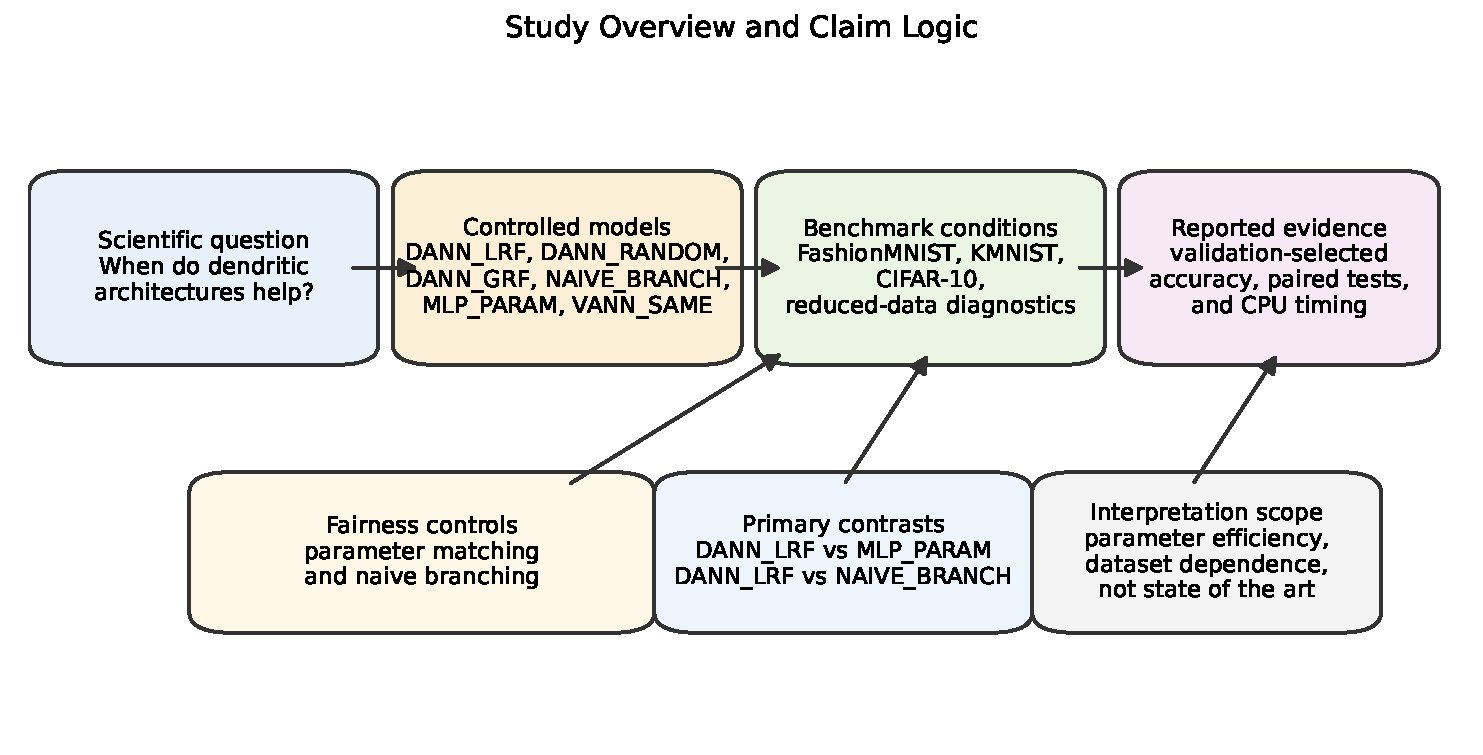
\includegraphics[width=\textwidth]{figures/fig_study_overview.pdf}
\caption{Study overview. The benchmark is designed around controlled contrasts rather than around absolute leaderboard performance. The main evidence combines validation-selected accuracy, seed-paired statistics, and CPU timing.}
\label{fig:overview}
\end{figure}

\subsection{DANN layer, routing strategies, and controls}
\label{sec:architecture}

Figure~\ref{fig:architecture} illustrates the layer logic shared by the DANN family. The formulation follows the general dendritic neuron modeling idea of local branch processing followed by soma-level aggregation \cite{todo2014unsupervised,gao2019dendritic,tang2024dnn,egrioglu2024deepdann}, but is intentionally simplified to support controlled benchmarking. Let $x \in \mathbb{R}^{D}$ denote a flattened input, $S$ the number of soma units, $B$ the number of branches per soma, $N = SB$ the number of dendrites, and $K$ the number of sampled features per dendrite. The model keeps a fixed routing tensor $I \in \mathbb{N}^{N \times K}$, sampled once at initialization and held fixed during training. Dendrite $n$ receives the subvector $x[I_n]$ and applies a local linear map followed by LeakyReLU:
\begin{align}
z_n &= \sum_{k=1}^{K} W_{n,k} x[I_{n,k}] + b_n, \\
a_n &= \mathrm{LeakyReLU}_{\alpha}(z_n).
\end{align}
The $B$ dendrites that belong to soma $s$ are then combined through cable weights:
\begin{align}
u_s &= \sum_{b=1}^{B} C^{c}_{s,b} \, a_{sB+b} + b^{s}_{s}, \\
h_s &= \mathrm{LeakyReLU}_{\alpha}(u_s), \\
y &= W^{o} h + b^{o}.
\end{align}

\begin{figure}[ht]
\centering
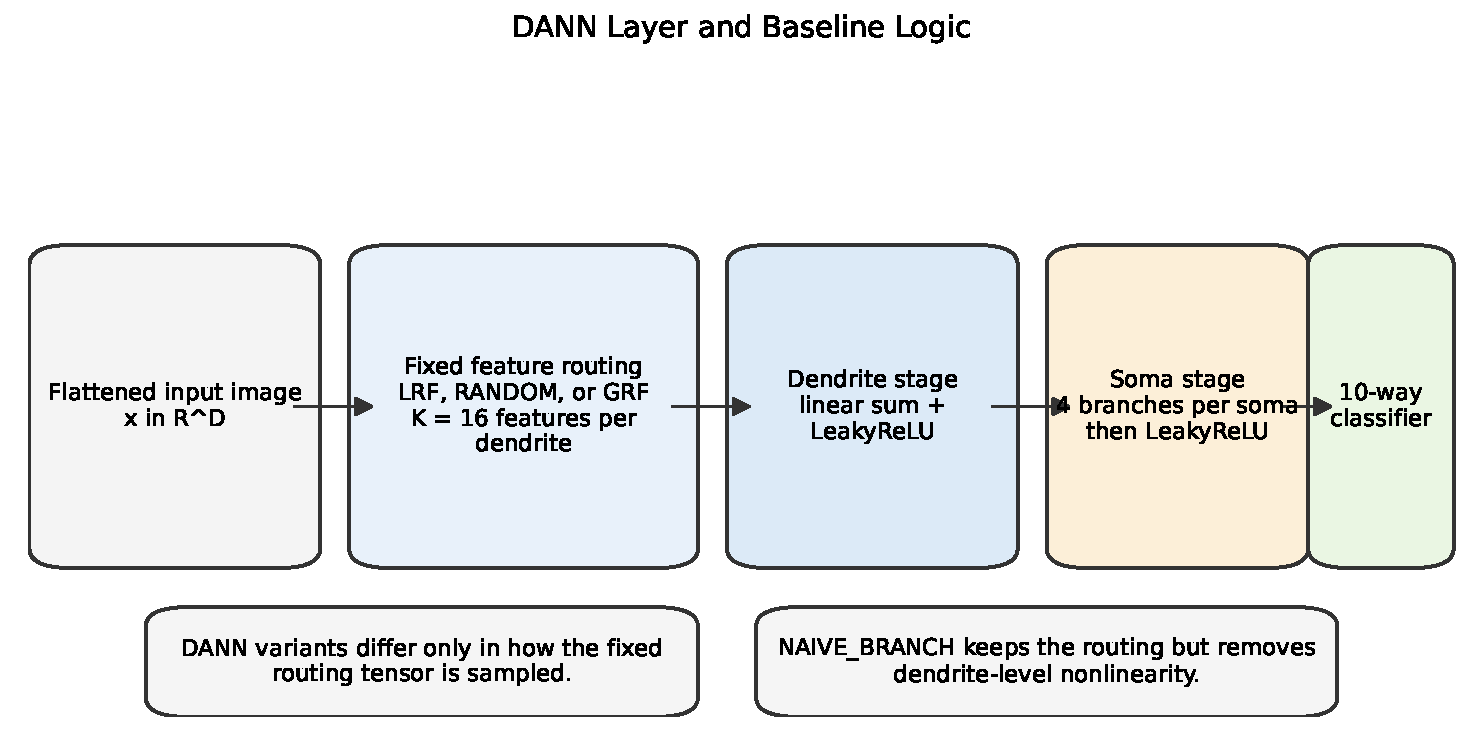
\includegraphics[width=\textwidth]{figures/fig_dann_architecture.pdf}
\caption{DANN layer and baseline logic. DANN variants differ only in how the fixed routing tensor is sampled. \NAIVEBRANCH{} keeps the same routed branch structure but removes the dendrite-level nonlinearity.}
\label{fig:architecture}
\end{figure}

Three routing strategies are evaluated.
\begin{itemize}
\item \DANNLRF: each dendrite samples $K=16$ features from a randomly placed $4 \times 4$ local patch. In CIFAR-10, the patch spans all three channels.
\item \DANNRANDOM: each dendrite samples $K=16$ features uniformly from the full flattened input.
\item \DANNGRF: all branches that feed the same soma share the same local patch, but each branch samples its own subset within that patch.
\end{itemize}

The baselines are chosen to isolate different explanations.
\begin{itemize}
\item \NAIVEBRANCH{} uses the same routed branch structure as \DANNLRF{} but removes dendrite-level nonlinearity before the soma stage.
\item \MLPPARAM{} is a two-hidden-layer multilayer perceptron whose width is selected to minimize parameter-count mismatch relative to the DANN model.
\item \VANNSAME{} is a wider two-hidden-layer dense network that serves as a high-capacity reference rather than as a parameter-matched baseline.
\end{itemize}

\subsection{Datasets, conditions, and archived scope}
\label{sec:datasets}

The study uses FashionMNIST, KMNIST, and CIFAR-10 as flattened-input ten-class image-classification tasks. Six archived accuracy conditions are available in the historical result package:
\begin{itemize}
\item FashionMNIST full
\item KMNIST full
\item CIFAR-10 full
\item FashionMNIST 0.2
\item FashionMNIST 0.1
\item CIFAR-10 0.2
\end{itemize}

The full-data FashionMNIST and KMNIST runs include all six low-parameter models plus \VANNSAME{}. The archived CIFAR-10 folders include \DANNLRF{}, \NAIVEBRANCH{}, \MLPPARAM{}, and \VANNSAME{}. The reduced-data folders focus on the main candidate method and its main controls; the archived CIFAR-10 0.2 folder also includes \VANNSAME{}.

An important historical detail is that the archived reduced-data runs were produced before the repository cleanup that separated training and test subsetting. In those historical folders, the same subset-fraction logic also affected the test loader. For that reason, the reduced-data results are treated in this manuscript as reduced-dataset diagnostics rather than as strict fixed-test low-training-data robustness experiments.

\subsection{Training protocol and parameter budgets}
\label{sec:protocol}

Table~\ref{tab:hyper} summarizes the shared hyperparameters and parameter counts. Unless otherwise noted, accuracy runs used 30 epochs, Adam \cite{kingma2015adam} with learning rate $10^{-3}$, batch size 256, and seeds $\{0,\dots,9\}$. Timing runs used 10 epochs, seeds $\{0,1,2\}$, and CPU-only execution. The archived accuracy runs were completed across mixed hardware contexts because they were collected in separate stages, but timing is reported only from the dedicated CPU protocol.

\begin{table}[ht]
\centering
\caption{Shared hyperparameters and parameter budgets.}
\label{tab:hyper}
\small
\begin{tabular}{ll}
\toprule
\textbf{Setting} & \textbf{Value} \\
\midrule
Soma units $S$ & 128 \\
Branches per soma $B$ & 4 \\
Dendrites $N=SB$ & 512 \\
Sampled features per dendrite $K$ & 16 \\
LRF/GRF patch size & $4 \times 4$ \\
Activation & LeakyReLU, slope 0.1 \\
Optimizer & Adam \\
Learning rate & $10^{-3}$ \\
Loss & Cross-entropy \\
Batch size & 256 \\
Epochs (accuracy runs) & 30 \\
Epochs (timing runs) & 10 \\
Accuracy seeds & $\{0,\dots,9\}$ \\
Timing seeds & $\{0,1,2\}$ \\
\midrule
DANN/NAIVE params (FashionMNIST, KMNIST) & 10,634 \\
\MLPPARAM{} params (FashionMNIST, KMNIST) & 10,527 \\
\VANNSAME{} params (FashionMNIST, KMNIST) & 468,874 \\
DANN/NAIVE params (CIFAR-10) & 10,634 \\
\MLPPARAM{} params (CIFAR-10) & 9,271 \\
\VANNSAME{} params (CIFAR-10) & 1,640,330 \\
\bottomrule
\end{tabular}
\end{table}

The FashionMNIST and KMNIST parameter mismatch between DANN and \MLPPARAM{} is about 1\%. On CIFAR-10 the mismatch is larger, about 14.7\% relative to \MLPPARAM{}, and should be kept in mind when interpreting parameter-efficiency claims on that dataset.

\subsection{Primary metric, paired statistics, and sensitivity audit}
\label{sec:metrics}

The historical summary CSV files export \texttt{best\_test\_acc}, which is the maximum test accuracy observed across epochs. Because that metric is test-selected, it is not used as the primary manuscript evidence. Instead, the manuscript reconstructs a validation-selected metric directly from the per-epoch history files: for each seed and model, we identify the epoch with the best validation loss and then report the test accuracy at that epoch. All tables and paired tests in the manuscript use this reconstructed metric.

For each condition, we computed paired Wilcoxon signed-rank tests \cite{wilcoxon1945individual} on seed-level validation-selected accuracies for the contrasts \DANNLRF{} versus \MLPPARAM{}, \DANNLRF{} versus \NAIVEBRANCH{}, and \DANNLRF{} versus \DANNRANDOM{} where available. Holm correction \cite{holm1979simple} was applied within each condition. We also report bootstrap 95\% confidence intervals on the mean paired difference using 10,000 resamples \cite{efron1994bootstrap}. This choice is consistent with standard recommendations for repeated classifier comparisons that avoid over-interpreting point estimates from a single split \cite{demsar2006statistical}. Finally, we performed a sensitivity audit comparing condition leaders under the historical best-test export and the reconstructed validation-selected metric.

\section{Results}
\label{sec:results}

All accuracy tables in this section report test accuracy at the best validation epoch, averaged across seeds. Historical best-test summaries are used only for the sensitivity audit discussed later. This distinction matters because it removes the main test-selection concern while preserving the available experimental evidence.

\subsection{Full-data benchmarks}
\label{sec:fullresults}

Table~\ref{tab:full} and Figure~\ref{fig:fullbars} summarize the three full-data conditions. The higher-capacity dense baseline, \VANNSAME{}, achieves the highest absolute accuracy in all three tasks, which is expected given its much larger parameter budget. The more informative question for this study is how the low-parameter models compare under matched or nearly matched capacity.

\begin{table}[ht]
\centering
\caption{Validation-selected accuracy on the three full-data benchmarks. Accuracy is reported as mean $\pm$ standard deviation across 10 seeds.}
\label{tab:full}
\small
\begin{tabular}{llrr}
\toprule
\textbf{Dataset} & \textbf{Model} & \textbf{Params} & \textbf{Accuracy (\%)} \\
\midrule
\multirow{6}{*}{FashionMNIST full}
& \VANNSAME{} & 468,874 & 88.72 $\pm$ 0.38 \\
& \DANNLRF{} & 10,634 & 87.03 $\pm$ 0.17 \\
& \DANNGRF{} & 10,634 & 86.86 $\pm$ 0.31 \\
& \NAIVEBRANCH{} & 10,634 & 86.67 $\pm$ 0.19 \\
& \DANNRANDOM{} & 10,634 & 86.48 $\pm$ 0.21 \\
& \MLPPARAM{} & 10,527 & 85.36 $\pm$ 0.27 \\
\midrule
\multirow{6}{*}{KMNIST full}
& \VANNSAME{} & 468,874 & 90.01 $\pm$ 0.36 \\
& \DANNRANDOM{} & 10,634 & 81.43 $\pm$ 0.34 \\
& \NAIVEBRANCH{} & 10,634 & 80.94 $\pm$ 0.45 \\
& \DANNLRF{} & 10,634 & 80.91 $\pm$ 0.62 \\
& \DANNGRF{} & 10,634 & 78.84 $\pm$ 0.37 \\
& \MLPPARAM{} & 10,527 & 76.85 $\pm$ 0.25 \\
\midrule
\multirow{4}{*}{CIFAR-10 full}
& \VANNSAME{} & 1,640,330 & 52.86 $\pm$ 0.69 \\
& \DANNLRF{} & 10,634 & 47.69 $\pm$ 0.55 \\
& \NAIVEBRANCH{} & 10,634 & 46.69 $\pm$ 0.31 \\
& \MLPPARAM{} & 9,271 & 30.65 $\pm$ 1.47 \\
\bottomrule
\end{tabular}
\end{table}

\begin{figure}[ht]
\centering
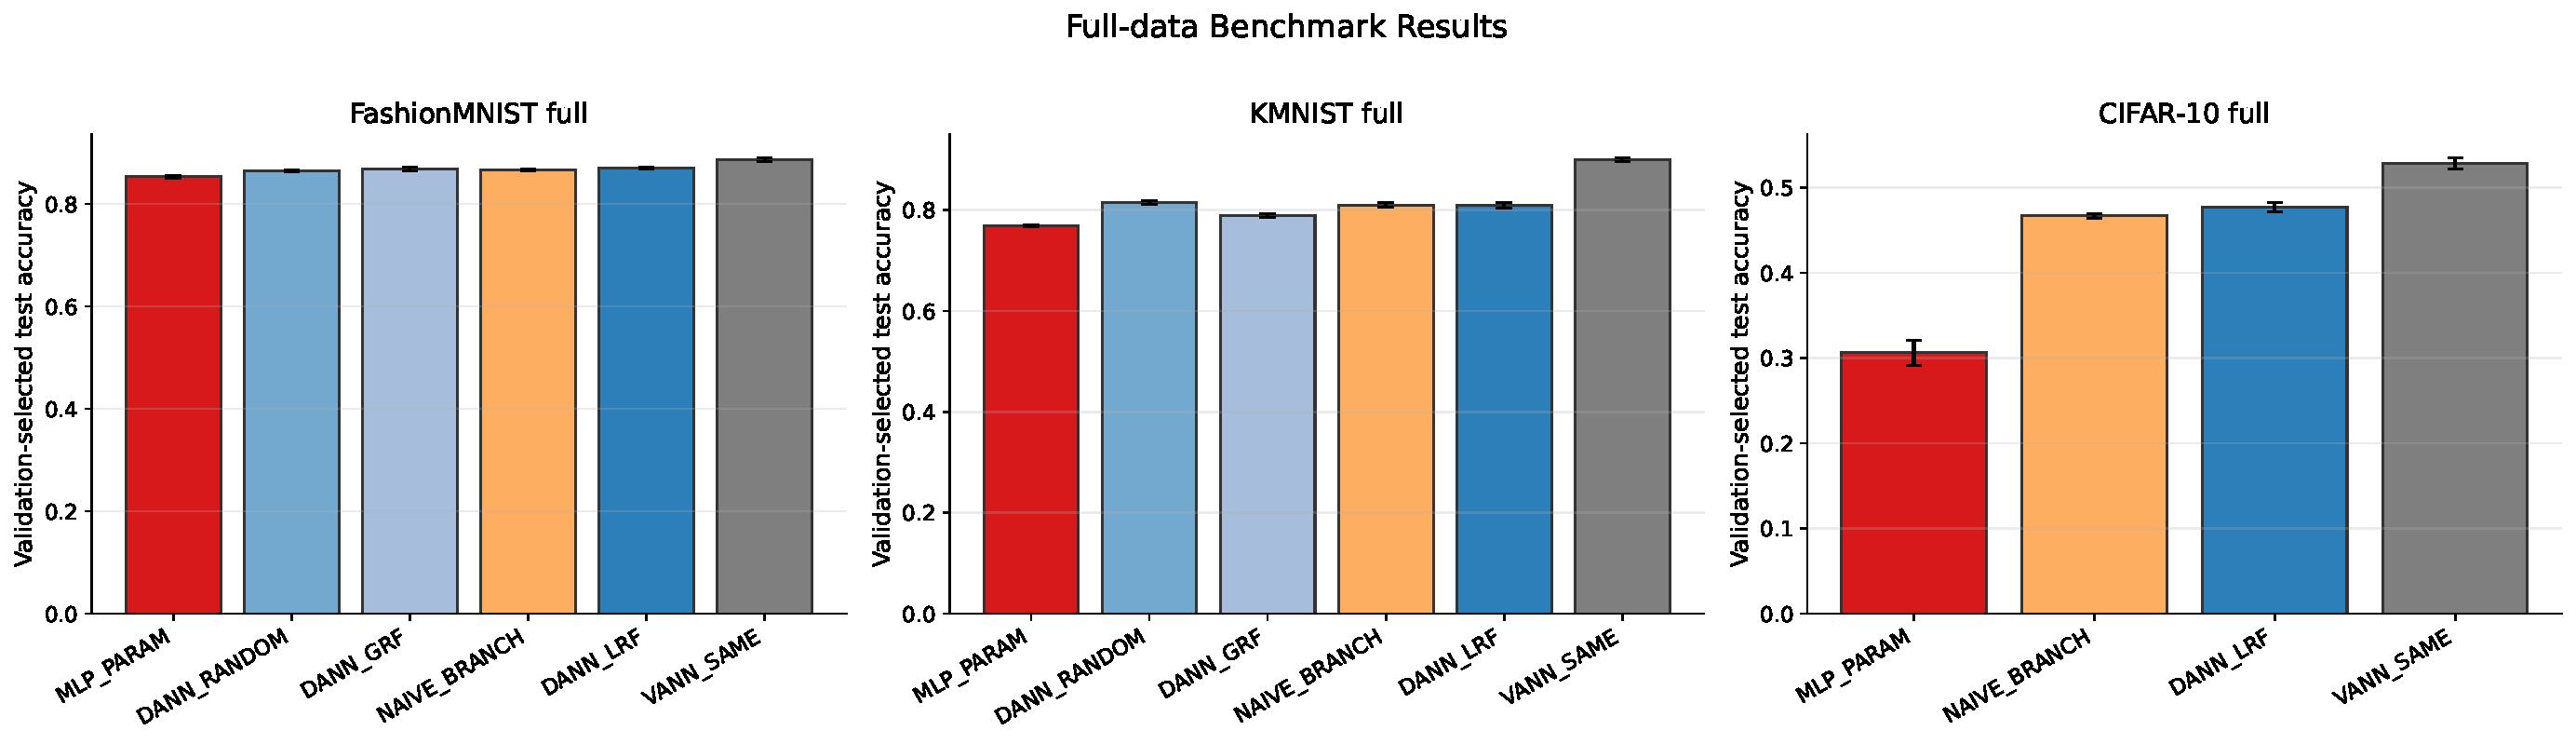
\includegraphics[width=\textwidth]{figures/fig_full_data_bars.pdf}
\caption{Validation-selected accuracy on the three full-data benchmarks. Error bars show seed-level standard deviation across 10 seeds.}
\label{fig:fullbars}
\end{figure}

The strongest full-data evidence is the consistent \DANNLRF{} advantage over \MLPPARAM{}. On FashionMNIST full, \DANNLRF{} exceeds \MLPPARAM{} by 1.67 percentage points, with a bootstrap 95\% confidence interval of [1.54, 1.80] and Holm-adjusted $p=0.0059$. On CIFAR-10 full, the gap grows to 17.04 points with Holm-adjusted $p=0.0039$. Even on KMNIST, where \DANNLRF{} is not the strongest DANN variant, it still exceeds \MLPPARAM{} by 4.06 points with Holm-adjusted $p=0.0059$.

The more demanding control is \NAIVEBRANCH{}. Here the effect is smaller and condition-dependent. \DANNLRF{} improves over \NAIVEBRANCH{} on FashionMNIST full by 0.37 points and on CIFAR-10 full by 1.01 points, both significant after Holm correction. On KMNIST, however, \DANNLRF{} and \NAIVEBRANCH{} are effectively tied, and the best DANN variant is \DANNRANDOM{} rather than \DANNLRF{}. This is a central result of the paper: dendritic computation can help, but the preferred routing strategy is not universal.

\subsection{Reduced-dataset diagnostics}
\label{sec:lowresults}

The historical reduced-data folders are informative, but they must be interpreted narrowly because the archival subset logic also reduced the test loader. Table~\ref{tab:low} and Figure~\ref{fig:lowbars} therefore present these runs as reduced-dataset diagnostics rather than as definitive low-training-data robustness evidence.

\begin{table}[ht]
\centering
\caption{Validation-selected accuracy on the archived reduced-dataset diagnostic runs. These folders were generated under historical subset logic that also affected the test loader.}
\label{tab:low}
\small
\begin{tabular}{llrr}
\toprule
\textbf{Condition} & \textbf{Model} & \textbf{Params} & \textbf{Accuracy (\%)} \\
\midrule
\multirow{3}{*}{FashionMNIST 0.2}
& \DANNLRF{} & 10,634 & 83.65 $\pm$ 0.79 \\
& \NAIVEBRANCH{} & 10,634 & 83.52 $\pm$ 0.86 \\
& \MLPPARAM{} & 10,527 & 83.21 $\pm$ 0.70 \\
\midrule
\multirow{3}{*}{FashionMNIST 0.1}
& \NAIVEBRANCH{} & 10,634 & 81.00 $\pm$ 0.78 \\
& \DANNLRF{} & 10,634 & 80.95 $\pm$ 0.89 \\
& \MLPPARAM{} & 10,527 & 80.94 $\pm$ 1.14 \\
\midrule
\multirow{4}{*}{CIFAR-10 0.2}
& \VANNSAME{} & 1,640,330 & 43.97 $\pm$ 1.24 \\
& \DANNLRF{} & 10,634 & 39.66 $\pm$ 0.83 \\
& \NAIVEBRANCH{} & 10,634 & 39.41 $\pm$ 0.77 \\
& \MLPPARAM{} & 9,271 & 26.48 $\pm$ 1.46 \\
\bottomrule
\end{tabular}
\end{table}

\begin{figure}[ht]
\centering
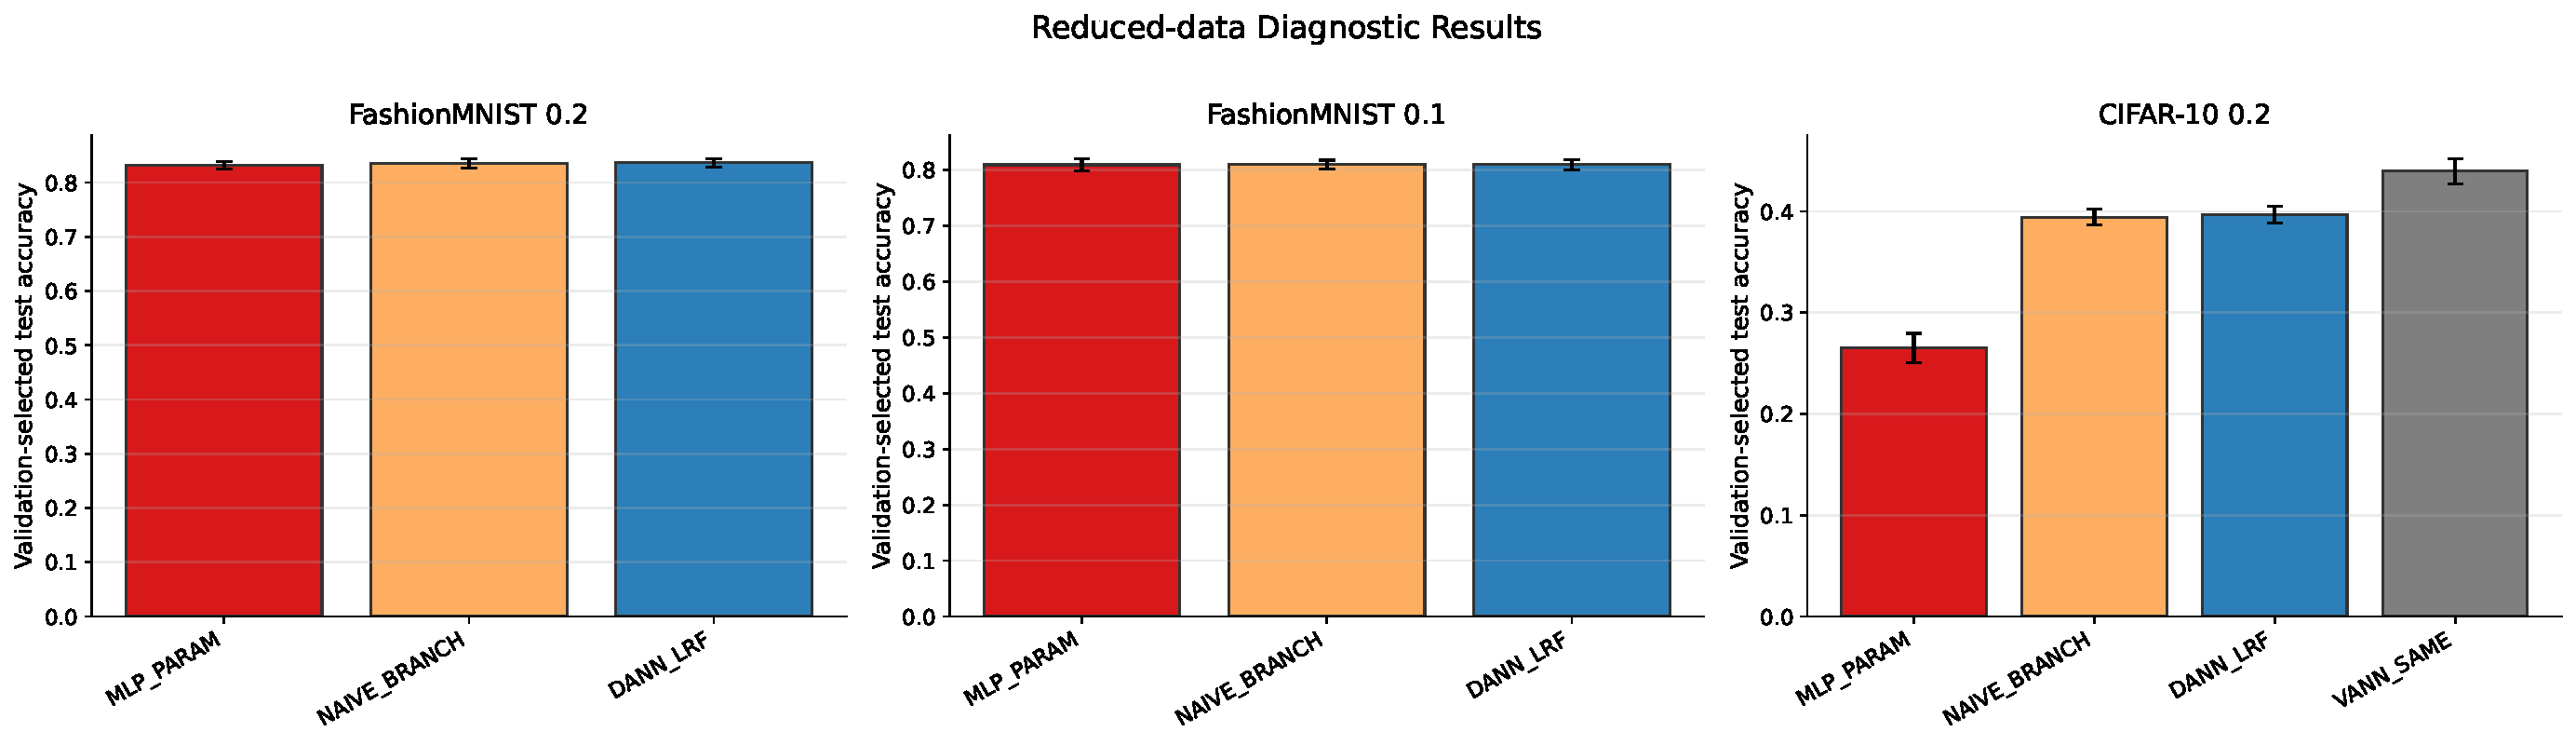
\includegraphics[width=\textwidth]{figures/fig_low_data_bars.pdf}
\caption{Validation-selected accuracy on the archived reduced-dataset diagnostic runs. Error bars show seed-level standard deviation across 10 seeds.}
\label{fig:lowbars}
\end{figure}

The reduced-dataset diagnostics are mixed. At the 20\% archived subset level, \DANNLRF{} remains numerically ahead of \MLPPARAM{} on both FashionMNIST and CIFAR-10, but only the CIFAR-10 gap is clearly large. FashionMNIST 0.2 shows a 0.44-point \DANNLRF{} advantage over \MLPPARAM{} and a 0.13-point advantage over \NAIVEBRANCH{}, neither statistically significant after Holm correction. FashionMNIST 0.1 is even less favorable to \DANNLRF{}: \NAIVEBRANCH{} ranks first, \DANNLRF{} is second, and neither contrast involving \DANNLRF{} is significant. In contrast, CIFAR-10 0.2 preserves a large \DANNLRF{} advantage over \MLPPARAM{} of 13.18 points, while the gap to \NAIVEBRANCH{} remains small and nonsignificant.

The evidence therefore supports a narrow reading: under the current archived reduced-dataset protocol, \DANNLRF{} retains some of its parameter-efficiency advantage in the moderate 20\% setting, especially on CIFAR-10, but the low-data story is not strong enough to support a general robustness claim.

\subsection{Paired contrasts and metric sensitivity}
\label{sec:paired}

Table~\ref{tab:paired} collects the primary paired contrasts, and Figure~\ref{fig:paired} visualizes the same effects with bootstrap confidence intervals. The pattern is consistent with the descriptive tables: large and reliable gains against \MLPPARAM{} on full-data conditions, smaller and condition-sensitive gaps against \NAIVEBRANCH{}, and a dataset-dependent preference within the DANN family.

\begin{table}[p]
\centering
\caption{Seed-paired statistical contrasts for \DANNLRF{} using validation-selected accuracy. Mean differences are reported in percentage points. Holm correction is applied within each condition.}
\label{tab:paired}
\scriptsize
\begin{tabular}{llrrr}
\toprule
\textbf{Condition} & \textbf{Contrast} & \textbf{Mean diff} & \textbf{95\% CI} & \textbf{Holm $p$} \\
\midrule
\multirow{3}{*}{FashionMNIST full}
& \DANNLRF{} $-$ \MLPPARAM{} & 1.67 & [1.54, 1.80] & 0.0059 \\
& \DANNLRF{} $-$ \NAIVEBRANCH{} & 0.37 & [0.26, 0.48] & 0.0059 \\
& \DANNLRF{} $-$ \DANNRANDOM{} & 0.55 & [0.41, 0.69] & 0.0059 \\
\midrule
\multirow{3}{*}{KMNIST full}
& \DANNLRF{} $-$ \MLPPARAM{} & 4.06 & [3.73, 4.37] & 0.0059 \\
& \DANNLRF{} $-$ \NAIVEBRANCH{} & $-$0.02 & [$-$0.35, 0.31] & 0.8457 \\
& \DANNLRF{} $-$ \DANNRANDOM{} & $-$0.51 & [$-$0.91, $-$0.13] & 0.0977 \\
\midrule
\multirow{2}{*}{CIFAR-10 full}
& \DANNLRF{} $-$ \MLPPARAM{} & 17.04 & [16.06, 18.12] & 0.0039 \\
& \DANNLRF{} $-$ \NAIVEBRANCH{} & 1.01 & [0.68, 1.34] & 0.0039 \\
\midrule
\multirow{2}{*}{FashionMNIST 0.2}
& \DANNLRF{} $-$ \MLPPARAM{} & 0.44 & [$-$0.04, 0.97] & 0.4922 \\
& \DANNLRF{} $-$ \NAIVEBRANCH{} & 0.13 & [$-$0.29, 0.53] & 0.4922 \\
\midrule
\multirow{2}{*}{FashionMNIST 0.1}
& \DANNLRF{} $-$ \MLPPARAM{} & 0.01 & [$-$0.43, 0.41] & 0.8457 \\
& \DANNLRF{} $-$ \NAIVEBRANCH{} & $-$0.04 & [$-$0.30, 0.26] & 0.8398 \\
\midrule
\multirow{2}{*}{CIFAR-10 0.2}
& \DANNLRF{} $-$ \MLPPARAM{} & 13.18 & [12.18, 14.23] & 0.0039 \\
& \DANNLRF{} $-$ \NAIVEBRANCH{} & 0.26 & [$-$0.54, 1.11] & 0.7344 \\
\bottomrule
\end{tabular}
\end{table}

\begin{figure}[ht]
\centering
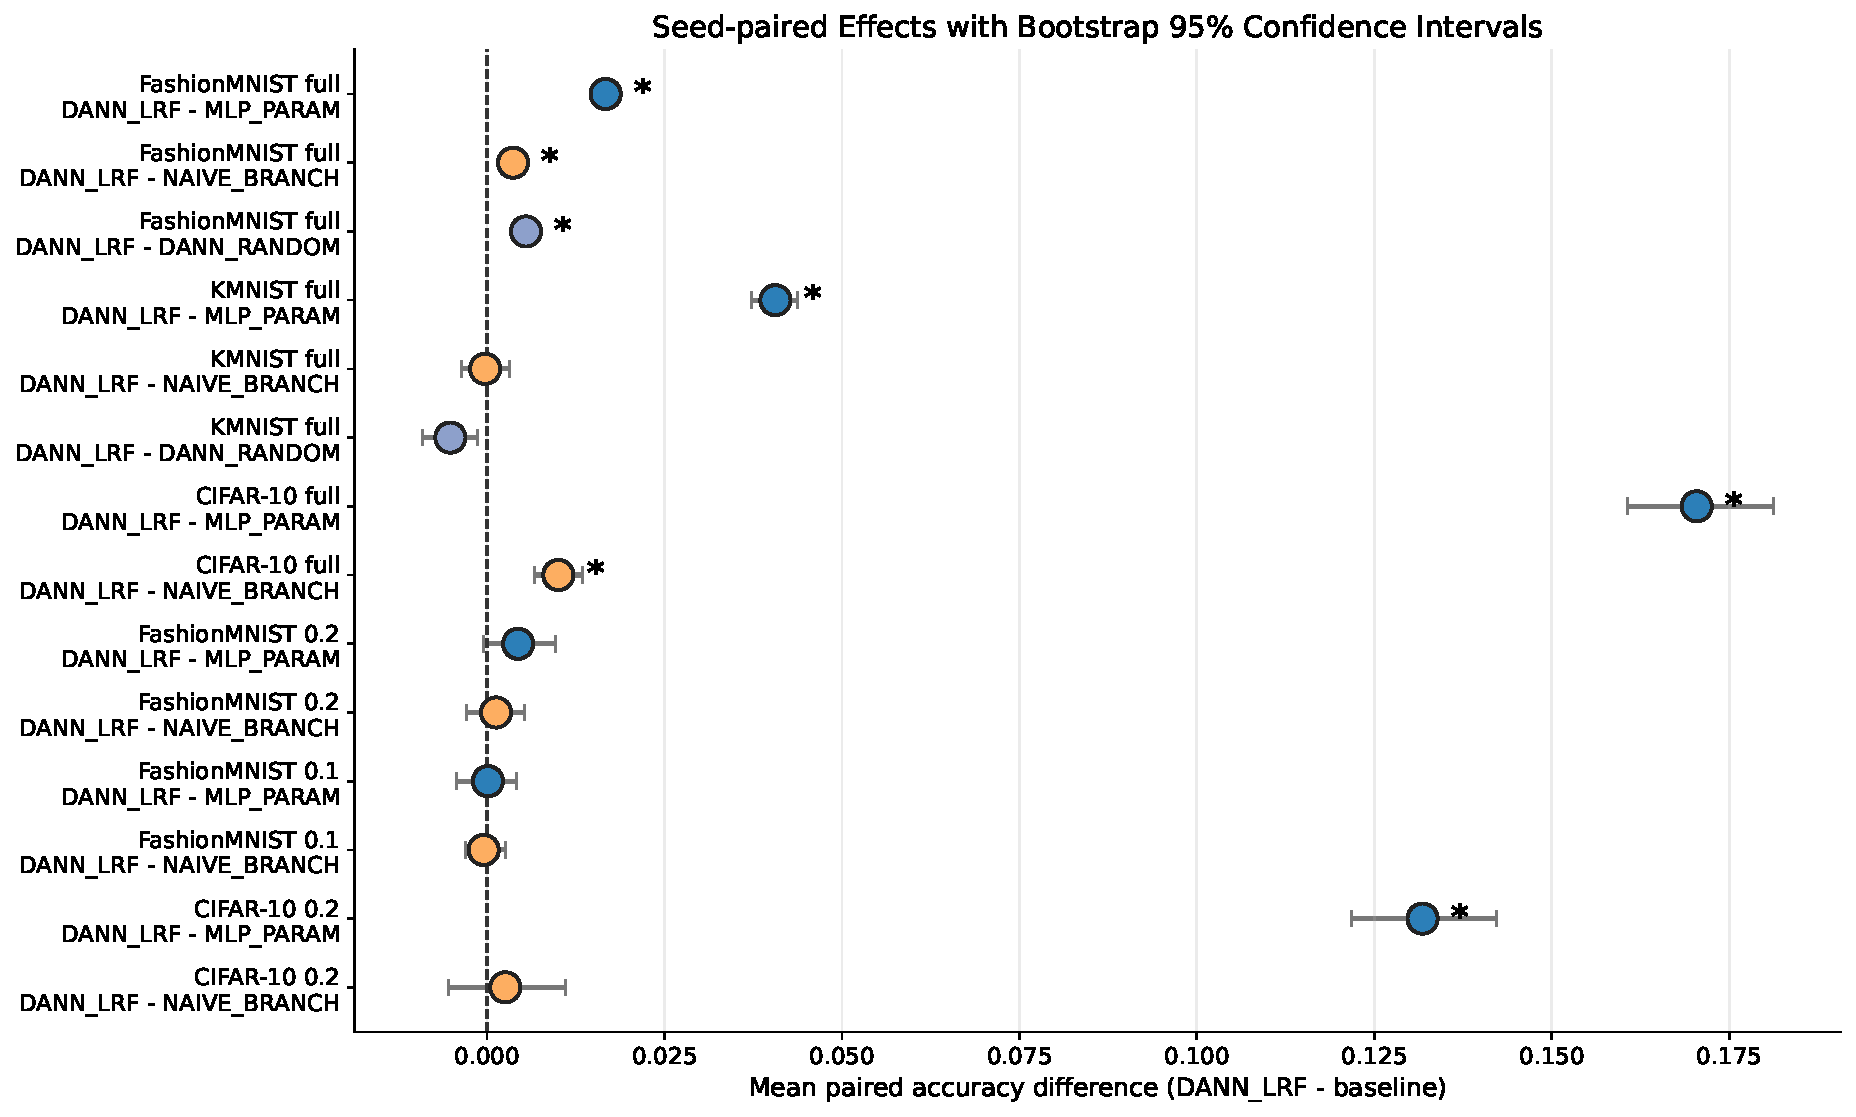
\includegraphics[width=\textwidth]{figures/fig_paired_diffs.pdf}
\caption{Seed-paired effects for \DANNLRF{} relative to its main baselines. Error bars denote bootstrap 95\% confidence intervals on the mean paired difference. Asterisks mark contrasts with Holm-adjusted $p < 0.05$ within condition.}
\label{fig:paired}
\end{figure}

The sensitivity audit is reassuring. When the historical best-test exports are compared with the reconstructed validation-selected metric, the leader of each condition is preserved. Lower-order rankings do change in a few places, especially between \DANNLRF{} and \NAIVEBRANCH{} on KMNIST and between \DANNLRF{} and \MLPPARAM{} on FashionMNIST 0.1, but the overall full-data narrative remains unchanged. This matters because it shows that the main claims are not artifacts of using a more conservative primary metric.

\subsection{CPU timing trade-offs}
\label{sec:timing}

The timing runs were carried out separately under a CPU-only protocol. Table~\ref{tab:timing} and Figure~\ref{fig:timing} show that \DANNLRF{} is consistently slower than \MLPPARAM{}, but only slightly slower than \NAIVEBRANCH{}.

\begin{table}[ht]
\centering
\caption{CPU-only timing summary from the dedicated timing runs. Accuracy values are included only as contextual outputs from the timing protocol and are not the main manuscript metric.}
\label{tab:timing}
\small
\setlength{\tabcolsep}{4pt}
\resizebox{\textwidth}{!}{%
\begin{tabular}{llrrrr}
\toprule
\textbf{Dataset} & \textbf{Model} & \textbf{Params} & \textbf{Acc. (\%)} & \textbf{Train s/epoch} & \textbf{Infer ms/1000} \\
\midrule
\multirow{4}{*}{FashionMNIST}
& \DANNLRF{} & 10,634 & 85.17 & 5.926 & 67.388 \\
& \MLPPARAM{} & 10,527 & 84.10 & 4.043 & 49.814 \\
& \NAIVEBRANCH{} & 10,634 & 84.58 & 5.756 & 66.706 \\
& \VANNSAME{} & 468,874 & 88.09 & 6.548 & 59.833 \\
\midrule
\multirow{4}{*}{CIFAR-10}
& \DANNLRF{} & 10,634 & 43.72 & 5.280 & 70.215 \\
& \MLPPARAM{} & 9,271 & 28.61 & 3.891 & 61.864 \\
& \NAIVEBRANCH{} & 10,634 & 42.82 & 5.095 & 67.961 \\
& \VANNSAME{} & 1,640,330 & 49.36 & 8.041 & 85.130 \\
\bottomrule
\end{tabular}
\par}
\end{table}

\begin{figure}[ht]
\centering
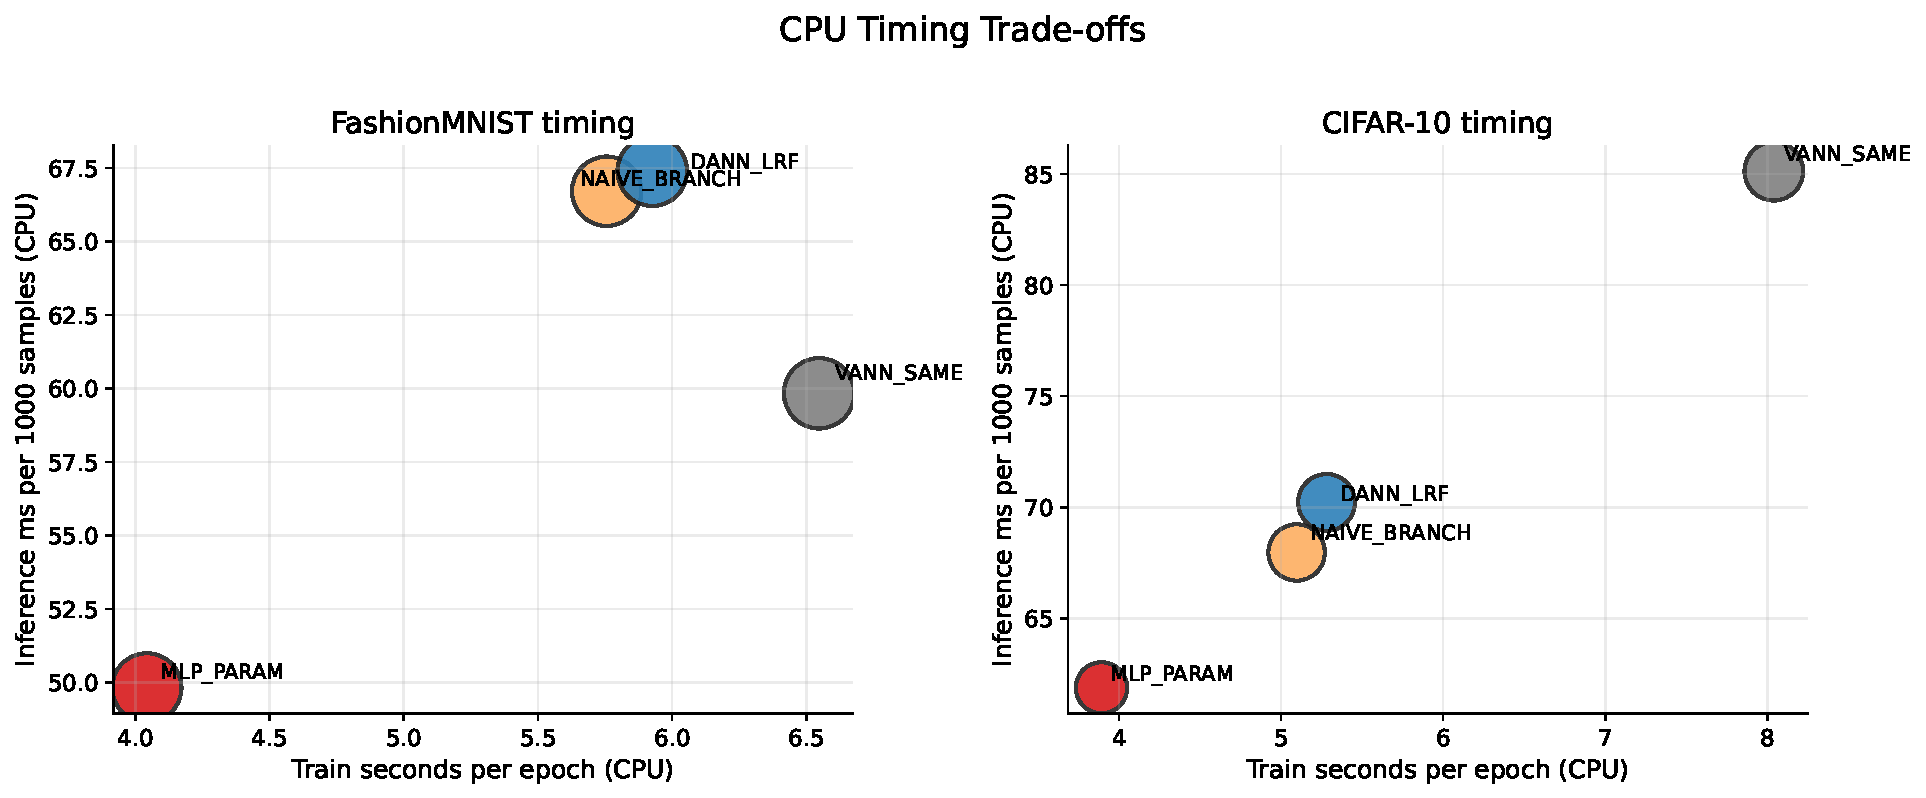
\includegraphics[width=\textwidth]{figures/fig_timing.pdf}
\caption{CPU timing trade-offs. Bubble area increases with timing-run accuracy, while the axes report training time per epoch and inference time per 1,000 samples.}
\label{fig:timing}
\end{figure}

Relative to \NAIVEBRANCH{}, \DANNLRF{} adds little cost: on FashionMNIST timing the overhead is 2.95\% in training and 1.02\% in inference, while on CIFAR-10 timing it is 3.63\% in training and 3.32\% in inference. Relative to \MLPPARAM{}, however, \DANNLRF{} is 46.59\% slower in training and 35.28\% slower in inference on FashionMNIST, and 35.70\% slower in training and 13.50\% slower in inference on CIFAR-10. The most defensible conclusion is therefore not that DANNs are cheap in absolute terms, but that the extra cost of dendritic nonlinearity beyond routed branching is modest.

\section{Discussion}
\label{sec:discussion}

The central finding is that dendritic structure improves parameter-efficient classification under several, but not all, benchmark conditions. Evidence for this claim is strongest in the full-data comparisons against \MLPPARAM{}. Across FashionMNIST, KMNIST, and CIFAR-10 full, \DANNLRF{} consistently exceeds the parameter-matched MLP, and the paired tests show that these gaps are not marginal. This supports the broader argument in the recent dendritic-computing literature that local branch processing can provide useful computational structure rather than merely biological ornamentation \cite{chavlis2021drawing,acharya2022dendriticcomputing,makarov2023efficiency,pagkalos2024leveraging,chavlis2025parameter}. In our benchmark, that value appears as a compact representational gain under a small parameter budget rather than as an absolute accuracy gain over large modern vision models.

The stronger scientific question, however, is whether the gain comes from dendritic computation itself or from branching alone. Here the answer is more nuanced. \DANNLRF{} beats \NAIVEBRANCH{} on FashionMNIST full and CIFAR-10 full, but the margins are much smaller than those against \MLPPARAM{} and they disappear on KMNIST and the most reduced FashionMNIST condition. This suggests that structured branching already explains part of the benefit, while dendrite-level nonlinearity contributes an additional but condition-sensitive increment. That distinction matters because adjacent efficiency work has also shown benefits from sparse routing, dendritic normalization, or structured connectivity even without our exact DANN formulation \cite{bird2021dendriticnorm,drix2018sparsecoding,fruengel2025sparseconnectivity,shaier2024moreexperts}. The present \NAIVEBRANCH{} control therefore helps separate two claims that are often conflated in the literature: branching can help, and dendritic nonlinearity may add further benefit, but the second claim must be tested against the first one directly.

Dataset dependence is the second major theme. On FashionMNIST, the local receptive-field prior appears well aligned with the underlying spatial regularity, and \DANNLRF{} is the strongest low-parameter model. On KMNIST, by contrast, \DANNRANDOM{} is numerically preferred, while \DANNLRF{} and \NAIVEBRANCH{} are effectively tied. A plausible interpretation is that KMNIST contains more distributed stroke relationships than the local-patch prior captures well. This is an interpretation rather than a proof of mechanism, but it is consistent with the broader lesson from recent dendritic ANN studies: routing strategy, dendritic interaction type, and task structure interact strongly, so no single dendritic design should be assumed to dominate across settings \cite{tang2024dnn,egrioglu2024deepdann,li2024alternating,liu2024capturecorr}. Our results therefore argue for dendritic architecture search under explicit controls, not for a universal local-receptive-field prior.

The CIFAR-10 results are scientifically useful even though the absolute accuracies are far below modern convolutional or transformer-based benchmarks. In a conventional computer-vision framing, these accuracies would be uncompetitive. In the present framing, however, CIFAR-10 acts as a harder stress test for shallow flattened-input models. Under that stress test, \DANNLRF{} clearly outperforms \MLPPARAM{} and improves over \NAIVEBRANCH{} on the full-data condition. The result therefore supports parameter efficiency, not state-of-the-art recognition. This positioning is important because some recent dendritic studies move directly toward deeper forecasting models, lightweight CNN variants, or hardware-aware spiking systems \cite{egrioglu2024deepdann,du2025shuffle,pagkalos2023dendrify,zheng2024temporal,dagostino2024denram}. A controlled shallow benchmark remains valuable precisely because it establishes what the architectural prior contributes before additional depth, convolution, recurrence, or neuromorphic machinery is introduced.

The reduced-dataset diagnostics should be interpreted conservatively. They suggest that \DANNLRF{} can retain some advantage in moderate reduction settings, especially on CIFAR-10 0.2, but they do not justify a strong low-training-data robustness claim because the historical archived protocol also affected the test loader. The negative FashionMNIST 0.1 result is therefore important and should remain visible in the paper. It shows that \DANNLRF{} is not universally favored under more severe data reduction. That negative result also prevents an overly optimistic reading of recent biologically inspired efficiency work \cite{bird2021dendriticnorm,chavlis2025parameter}: dendritic inductive bias can help, but its benefits remain regime-dependent and should be stated with the same caution as its successes.

Another useful implication concerns architecture versus learning rule. A major branch of biologically plausible learning research studies segregated dendrites, predictive coding, feedback control, and local credit assignment as alternatives or complements to standard backpropagation \cite{guerguiev2017segregated,meulemans2021deepfeedback,tang2023predictive,millidge2024temporal,lv2025localized}. Our study does not address that learning-rule question. Instead, it shows that even under ordinary supervised optimization, the neuronal architecture itself can inject a measurable inductive bias. This suggests that dendritic architecture and biologically plausible learning rules should be treated as complementary research directions rather than as mutually exclusive explanations. A future system could combine the architectural controls used here with compartment-aware credit-assignment schemes to test whether the two sources of inductive bias are additive.

Finally, the timing analysis clarifies the computational trade-off. \DANNLRF{} is not free. It is clearly slower than \MLPPARAM{} in both training and inference. Yet the additional cost beyond \NAIVEBRANCH{} is small, which means that most of the compute cost comes from routed branching itself, not from adding the dendrite-level nonlinearity on top of that structure. This makes \DANNLRF{} a plausible candidate when the research goal is to trade modest runtime overhead for higher accuracy under a small parameter budget. That conclusion also aligns with the recent framing of dendrites as efficiency-oriented computational resources rather than as gratuitous biological embellishments \cite{makarov2023efficiency,pagkalos2024leveraging,chavlis2025parameter}.

\section{Limitations and Reproducibility Notes}
\label{sec:limitations}

Several limitations should be stated explicitly.
\begin{enumerate}
\item All models operate on flattened image inputs. The study does not compare against convolutional backbones, residual networks, or transformers, and it should not be read as a modern vision benchmark.
\item \VANNSAME{} is a high-capacity reference, not a fair parameter-matched competitor. Its higher absolute accuracy does not invalidate the parameter-efficiency question, but it does bound how much can be claimed about absolute performance.
\item The archived reduced-data folders were generated before the train-subset and test-subset logic were cleanly separated in the repository. They are therefore presented as reduced-dataset diagnostics, not as strict fixed-test low-training-data evidence.
\item The historical summary CSV files export best test accuracy across epochs. To avoid test-set selection bias, the manuscript reconstructs the primary metric from per-epoch histories and uses test accuracy at the best validation epoch instead.
\item The archived accuracy runs were completed across mixed hardware contexts. This does not undermine the accuracy comparisons themselves, but it means that wall-clock interpretation must rely on the dedicated CPU timing protocol rather than on the accuracy folders.
\item The archived result package predates the repository-side fix that now sets all seeds before model construction. The historical outputs remain usable, but this detail slightly weakens strict rerun-level determinism for those archived folders.
\item The CIFAR-10 folders in the archived package evaluate \DANNLRF{} against controls, but they do not include \DANNRANDOM{} or \DANNGRF{}. As a result, the dataset-dependence conclusion about routing strategy is strongest for FashionMNIST and KMNIST.
\end{enumerate}

These limitations do not invalidate the main full-data findings. They instead define the scope of the evidence: controlled, shallow, parameter-aware benchmarking of dendritic architectures, with especially strong support for the full-data comparisons and more cautious support for the archived reduced-data diagnostics.

\section{Conclusion}
\label{sec:conclusion}

This study asked a narrow but important question: when do dendritic artificial neural networks help once parameter count, branching structure, and runtime are controlled? The answer is favorable but not universal. \DANNLRF{} consistently improves over a parameter-matched MLP on the full-data benchmarks and on archived CIFAR-10 0.2, while its advantage over naive branching is smaller and condition-dependent. The preferred routing strategy is dataset-dependent, with local receptive fields favored on FashionMNIST and random routing numerically favored on KMNIST. CPU timing shows that the extra cost of dendritic nonlinearity beyond branching is modest, although \DANNLRF{} remains slower than the plain MLP baseline. Taken together, the results support DANNs as parameter-efficient classifiers whose value lies in controlled architectural trade-offs rather than in universal accuracy maximization.

\section*{CRediT authorship contribution statement}

{\"O}zkan Canay: Conceptualization, methodology, software, validation, formal analysis, investigation, visualization, writing - original draft, writing - review and editing.

\section*{Declaration of competing interest}

The author declares that there are no known competing financial interests or personal relationships that could have appeared to influence the work reported in this paper.

\section*{Data availability}

The codebase, archived historical outputs, manuscript-derivation scripts, and generated tables and figures are prepared for public release at \url{https://github.com/canay/dendritic-ann-benchmarks}. Dataset access notes and source links for FashionMNIST, KMNIST, and CIFAR-10 are documented in the repository so that reviewers can reproduce downloads from the original dataset providers. The manuscript tables were reconstructed from per-epoch history files to report validation-selected test accuracy as the primary metric.

\bibliographystyle{elsarticle-num}
\bibliography{refs,refs_expanded}

\end{document}
